\chapter{Geology of Migovec}

\section{The Julian Alps}
\label{sec:The Julian Alps}

\subsection{Geography} 
\label{par:Geography} 
\passage{Tolminski Migovec} belongs to the \passage{Julian Alps}, in the easternmost sector of the \passage{Southern Alps} \citep{bavec2004late}. 
They \passage{Julian Alps} are bounded by the Pannonian and  Fruili-Veneto basins to the east and west respectively, while to the north, they are separated from the \passage{Eastern Alps} by the Periadriatic lineament (\fref{map:geol large scale}). Southward from the South Alpine front, they become the \passage{Dinarides} \citep{placer1998contribution,burrato2008sources}.
This carbonate dominated massif is characterised by high relief with valley floors located 100-400\,m asl and peaks in excess of 2000\,m asl  \citep{vsmuc2009tectonic}. 

\subsection{Structural style}
\label{par:Structural style}
Overall, the tectono-stratigraphic setting \sidenote{The interplay between relief generation, erosion and sedimentary deposition during \emph{orogenesis} or moutain building events} of the \passage{Julian Alps} is a result of continued northward motion of about 2\,mm.a$^{-1}$ \citep{burrato2008sources} and since the Miocene,  counter-clockwise rotation of the Adriatic microplate \citep{marton2003palaeomagnetic}. 
The convergence of the Adria microplate with the Eurasian plate is quantitatively described by GPS velocity fields \citep{grenerczy2005tectonic}. 
Such convergence has led to the formation of Alpine and Dinaric mountain chains and still generates earthquakes today ($M_w$ > 5) in the parts of the shallow crust where shortening is accommodated by brittle deformation.

Slovenia, and in particular the area north east of Tolmin are located in the north-eastern corner of the Adria-Europe collisional belt. 
This area, at the critical juncture between the Alpine and Dinaric chains overlook a rim of high topography around the relatively rigid, undeformed Adria micro-plate, whose rocks are  exposed in the Istrian (West Croatia) peninsula \citep{vsmuc2009tectonic}. 
It is buried under a thick cover of foredeep \sidenote{Foredeep basins form in the immediate vicinity of collisional belt as thickened crust deforms the somewhat elastic plate underneath, creating a trough where the material sourced from the nearby mountains is preferentially deposited}sediments in the Friuli-Venetian plain. 

It is useful to define a hierarchy for the subdivision of tectonic units within the Tolmin area. 
At first order, the \passage{Southern Alps} lie between by the Periadriatic lineament and South Alpine front \citep{placer1998contribution}. 
Second order units, e.g. the Zlatna, Julian (locally Krn) and Tolmin nappes are slices bounded by south verging thrust faults. 
This reverse thrusting resulted in an inversion of stratigraphical order, which places massive upper Triassic limestones at the top of the sequence with younger Jurassic/Cretaceous marls and limestones outcropping underneath, at much lower elevation (\fref{map:mapofgeology}).

\begin{map}[b!]
\checkoddpage \ifoddpage \forcerectofloat \else \forceversofloat \fi
\includegraphics[width = \textwidth]{images/maps-of-mig/geology_large.png}
\caption[Structural setting of NW Slovenia]{\emph{(a)} Overview map of Slovenia \emph{(b)} The structural setting of northwestern Slovenia shows the \protect\passage{Tolmin} area straddling the active \protect\passage[fault]{Idrija} and \protect\passage[fault]{Ravne} faults. The \protect\passage{Migovec System} is developed within the Slatna overthrust and the underlying Dachtsein limestone. Inset C is shown in the geological map from \citet{buser1986tolmavc}. Figure modified from \citet{vsmuc2009tectonic} and \citet{celarc2014new}}
\label{map:geol large scale}
\end{map}


 
\subsection{Alpine deformation}
\label{par:alpine deformation}
That the \passage{Julian Nappe}, which comprises the cave forming Dachstein Formation of the \passage{Krn}-\passage{Migovec} area was transported towards the south during the Alpine orogen is commonplace in the litterature \citep{doglioni1987eoalpine,placer1998contribution}. 
The weak and easily deformed Carboniferous clastics basement of the \passage{Julian Alps} provided a detachment horizon along which the nappe was transported from the north southwards. The question of the timing of transport of this nappe is somewhat more difficult. \citet{buser1986tolmavc} attributes a Neogene (~23\,Ma to 3\,Ma BP) age to this tectonic structure, while \citet{placer1998contribution} argues it could be slightly older, starting in mid to Late Oligocene (28\,Ma BP).

\subsection{Present day stress regime}
\label{par:present day stress regime}
The activity on this heavily faulted boundary between Adria and Eurasia is highlighted by recent destructive earthquakes: $M_w$=6.4 on the Italian side in 1976 \citep{pondrelli2001seismotectonic}, and $M_w$=5.7 and $M_w$=5.2 on the Slovenian side in 1998 \citep{bajc20011998} and 2004 \citep{aoudia2005july} respectively. 
To highlight the vulnerability of this region, it is also worth keeping in mind that the largest earthquake ever at this junction between the \passage{Southern Alps} and the \passage{Dinarides} was the 1511 western Slovenia earthquake ($M_w$= 6.8). It is believed to have resulted in at least 12,000 deaths \citep{fitzko2005constraints}.
Fault plane solutions for the many $M_w$=4-6 regional quakes demonstrate that the mode of deformation on the Italian side is chiefly by thrusting \citep{poli2002new}, while deformation is accommodated by dextral slip on the Slovenian side \citep{poljak2000seismotectonic}. 
The main strike-slip faults in NW Slovenia i.e. the \passage[fault]{Idrija}, \passage[fault]{Ravne} and \passage[fault]{Sava} faults from south to north have a spectacular topographic expression. 

\begin{figure}[t!]
\checkoddpage \ifoddpage \forcerectofloat \else \forceversofloat \fi
\centering
\frame{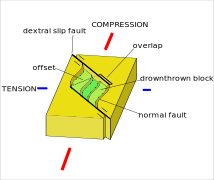
\includegraphics[width =\textwidth]{images/maps-of-mig/faultblock.png}}
\caption{A simplified block diagram showing development of a pull apart basin. Redrawn from \citet{WU20091608}}
\label{fig:fault}
\end{figure}

The \passage[fault]{Ravne} and \passage[fault]{Idrija} faults' expression was mapped by \citet{cunningham2006application} with the aid of LiDAR data. The \passage[fault]{Ravne} fault is actively growing and supports dextral slip motion through right stepping segments \citep{kastelic2008neo}.
This results in local transtensional stress regimes which generate steep normal faults which are involved in building the topography between \passage[town]{Bovec}, through to \passage{Ravne}. 


Seismic source modelling suggests a 13\,km  segment was involved in the 1998 earthquake, therefore it is possible that this fault generated stronger earthquakes in the past; it is thought it was involved in the devastating 1511 earthquake \citep{fitzko2005constraints}.
On the geological map the NW-SE trending fault passes to the NE of \passage{Krn}, between \passage{Gru\v{s}nica} and \passage{Tolminski Migovec} and heads towards \passage{Tolminske Ravne} hamlet (\fref{map:mapofgeology}).

Crucially, the \passage{Ravne} fault segments pass through the \passage{Tolminka} springs basin, and its Quaternary (3\,Ma to Present) activity has played a primary role in the building local topography of the \passage{Tolminka} valley (±1200\,m relief), which is described as a small pull-apart basin 2.1\,km long and 510\,m wide \citep{cunningham2006application,kastelic2008neo}. With respect to \fref{fig:fault}, the overlap between the two segments of the \passage{Ravne} fault is ~370\,m and their offset is ~300\,m. The total topographic lowering related to fault activity during the last 3\,Ma is ~1200\,m.

In short this basin highlights the interplay between old Alpine structures, recent cross-cutting faults, glacial and hillslope erosional processes and karst development.

\subsection{Summary of tectonic history}
\label{par:summary of tectonic}
\citet{kastelic2008neo} recognise three main phases of tectonic activity with topographic and clear structural expression within the \passage{Southern Alps}.

\begin{citemize}
\item Dinaric reverse thrusting within the Eocene (56\,Ma-33\,Ma BP). Reverse faults with orientations NW-SE orientations develop  \citep{castellarin2000neo}.
\item South Alpine thrusting transport of the Mesozoic carbonate platforms which form the \passage{Julian Alps} as described by \citet{placer1998contribution} and \citet{buser1986tolmavc} from possibly mid-Oligocene to mid-Miocene. The resulting compressional tectonic structures are mostly E-W oriented \citep{castellarin2000neo}.
\item Neogene (Pliocene to Recent) dextral-slip faulting cross-cutting the Alpine generated topography, producing youthful landforms such as the \passage{Tolminka} springs basin, continuing today, highlighted by earthquake activity \citep{vsmuc2009tectonic,cunningham2006application}.
\end{citemize}

 \begin{pagemap}
 \checkoddpage \ifoddpage \forcerectofloat \else \forceversofloat \fi
\centering
  \includegraphics[width=\textwidth]{"images/maps-of-mig/final_geology".png}
  
  \caption{Geological map of the \passage{Tolmin} Area, modified after \citet{buser1986tolmavc}}
  \label{map:mapofgeology}
 \end{pagemap}

\section{Landscape development and controls}
\subsection{Lithology}
\label{par:lithology}

The \passage{Migovec} cave system is formed principally in well stratified and heavily faulted Dachstein Formation. These highly permeable and well karstified limestones were deposited on the Julian carbonate platform \citep{ogorelec1996dachstein}.
The carbonates, which also contain patches of dolomite, form a continuous sequence reaching nearly km thick \citep{buser1986tolmavc}.
In cave observations of well exposed canyon and shaft walls suggest that at least part of the sequence is made up of alternating carbonate facies e.g. light grey mudstone, cream to grey horizons of wackestones containing fossil algae, mud clasts and gastropod shells (e.g. in \passage{Hall of the Mountain King},\fref{fig:hotmk2}). 
The light grey beds are likely a deeper lagoonal facies, while the cream-coloured beds were deposited closer to the reefs. 
Light grey horizons are often 1-2 m thick, while the cream-coloured facies are usually  made up 0.5 m thick beds. 

Although coral reef buildups have been recognised in the surrounding areas \citep{buser1986tolmavc,ogorelec1996dachstein}, none have been reported so far in the Migovec cave system. 

The underlying formation of bedded to massive dolostone (the Main Dolomite Formation) is shown to outcrop on the NE side of the Tolminka valley on the geological map of \passage{Tolmin} \citep{buser1986tolmavc}.
 This formation, less karstified than the overlying Dachstein Formation, acts as a local aquiclude, as is shown for the Kanin massif whose geological context is similar \citep{turk2015hydrogeological}. 

\marginnote{\emph{Lithology} describes the summary of the gross characteristics of a rock}
The rock formed during the Upper Triassic Norian to Rhaetian age (228 -101.3\,Ma) and now forms the backbone the \passage[Calcareous Alps]{Southern Calcareous Alps} \citep{bosellini1974triassic} and crops out all over the \passage{Northern Calcareous Alps} \citep{fischer1975tidal,schwarzacher2005stratification}. It has given rise to spectacular landscapes spread over Southern Europe, from Hungary \citep{haas2004characteristics} to Sicily \citep{catalano1974ciclotemi}.
Its ubiquity has wide ranging implications for the palaeogeography of this region in Norian to Rhaetian times.

The deposition of the Dachstein Formation ended at the end of the Triassic ($\approx200$\,Ma BP) with the dislocation of the carbonate platform. Some regions stayed near the sea level (the so-called 'Julian High') while others were periodically drowned, leading to a loss of carbonate productivity and the deposition of mudstones and shales within the limestone sequence, at  Jurassic and Cretaceous \citep{vsmuc2010jurassic} times; they are shown on \fref{fig:limestones and marls}.

\begin{marginfigure}
\frame{\includegraphics[width = \textwidth]{images/maps-of-mig/dachstein_limestone.jpg}}
\caption{The well bedded Dachstein Formation outcrops on the western cliffs of \passage{Tolminski Migovec} \pic{Rhys Tyers}}
\label{fig:dachstein}
\end{marginfigure}

Debate is ongoing as to the origin of the cyclic pattern of the limestone beds often called \emph{Lofer cyclothems} --- so named after the Lofer locality in Austria where they were first described. 
These cyclothems were identified and interpreted by \citet{fisher1964lofer} as cyclic sequences tracking deepening upwards depositional environments.
The idealised cyclothem model shows three groups A, B, C corresponding to  subaerial, tidal and subtidal deposition environments respectively.  

This is demonstrated by palaeokarst solution vugs, the presence of argillaceous --- here terrestrially derived --- and often iron oxide rich residues and evidence of subaerial weathering, even palaeokarst in Group A.

Group B is often characterised by the presence of dessication cracks, partial dolomitisation; it is often laterally discontinuous, with variable thicknesses (5-155\,cm).

Group C, often the most abundant, comprises wackestones (limestones rich in carbonate mud) and packstones (dominated by biogenic fragments).

Often, the measured sections differ from the ideal model by the absence of certain members of the sequence. Indeed compared with the Dachstein formation deposited in the Dinaric range, the limestones of the \passage{Krn} area show more numerous and more pronounced periods of local emersion \citep{ogorelec1996dachstein}.

 With some authors favouring local tectonic control as a causal mechanism  for relative changes in sea level \citep{goldhammer1990depositional,enos1998lofer}, others \citep{fisher1964lofer,balog1997shallow,haas2004characteristics,doi:10.1130/G21578.1}, prefer orbitally forced environmental fluctuations such as \emph{Milankovitch cycles} which result from periodic fluctuations in solar insolation linked with the Earth's \emph{precession}, \emph{tilt} and \emph{ellipticity} cycles. 



 \subsection{Glacial landforms}
 \citet{bavec2004late} used a combination of geological mapping and dating the identified glacial deposits in order to constrain the extent of late Quaternary glaciation in the upper So\v{c}a valley, which is relevant to the Tolmin area.

 Most notably, they find no clearly expressed glacial geomorphic features downstream of the town of Bovec; on the contrary, all landforms such as end moraines or glacial cirques are limited to the high reaches on the valleys. 

Locally, the bowl shaped hanging valley between the \passage{Migovec Plateau} and \passage{Vrh Nad \v{S}krbino} is one example of glacial cirque. Notably, the high resolution mapping of \citet{cunningham2006application} could not find any signes of side or end moraine, nor any other glacially derived deposits within the \passage{Tolminka} springs basin and interpreted the sheer walls near \passage{Polog} as segments of the \passage{Ravne} fault in a pull-apart basin. 
This is consistent with the view of \citet{vsmuc2009tectonic} on the relative primacy of tectonics over glacial processes on landscape building in the \passage{Triglav} area.

\begin{marginfigure}
\checkoddpage \ifoddpage \forcerectofloat \else \forceversofloat \fi
\centering

 \frame{\includegraphics[width=\linewidth]{"images/maps-of-mig/marls_limestone".jpg}} 
 \caption{An example of the Jurassic marl and limestone succession, which is heavily faulted \pic{Tanguy Racine}, on the \protect\passage{Slovenska Geolo\v{s}ka Pot}}
 \label{fig:limestones and marls}
\end{marginfigure}


 \section{A Karstic landscape}
Karst terrain arises from the combination of high rock solubility and well developed secondary fracture porosity \citep{ford2013karst}. 

Such terrains exhibit several key features: fluted outcrops, sinks, caves, springs, blind valleys etc... These landforms are generated by the dissolution of rock along natural subterranean pathways provided by geological features (joint, bedding planes, faults). The chemical pathways and rates of fissure enlargement are described in detail in \citet{dreybrodt1996principles}.

\begin{figure}[t!]
\checkoddpage \ifoddpage \forcerectofloat \else \forceversofloat \fi
\frame{\includegraphics[width = \textwidth]{images/maps-of-mig/limst_bedded_folded_jana_08.jpg}}
\caption{A closed depression on the \passage{Migovec Plateau}, where the bedding dip and fold patterns controls the geometry of the snow pit. The differential erosion of the limestone strata leads thinly bedded, more heavily fractured horizons to provide a disproportionate amount of frost-shattered debris to the scree cone.  \pic{Jana \v{C}arga}}
\label{fig:closed_depression}
\end{figure}

Shakehole dolines and closed depressions of varying size (5-50\,m diameter) riddle the \passage{Migovec Plateau} surface \fref{map:map overlay}. The majority are between 10 and 3\,m deep and contain snow plugs. Shakeholes are distributed preferentially along lines of fractures and develop at the intersection of those fracture sets \fref{map:mapofgeology}. The large closed depressions are theatre-shaped, with clear bedding control on the development of scree and cliff. This results in a pattern of depressions with 5-20\,m rock cliffs to the south, and scree slopes to the north.

Bedding control of karst development is seen north of \passage{Tolminski Migovec}, in an area of well developed Schichttreppen karst. Locally the bare limestone beds outcrop as a succession of inclined surfaces, where fractures were enlarged by bedrock dissolution to form deep, snow-filled fissures. The east slope of the \passage{Tolminski Migovec} plateau is developed in a staircase pattern, with bedding surfaces sloping to the southwest and joints or vertical fractures surfaces sloping to the northeast (\fref{fig:karstic_landscape}).

\begin{pagefigure}
\checkoddpage \ifoddpage \forcerectofloat \else \forceversofloat \fi
\frame{\includegraphics[width = \textwidth]{images/maps-of-mig/western_cliffs.jpg}}
\caption{ A view of the \passage{Tolminski Migovec} plateau, towards the south, as seen from the summit of \passage{Tolminski Kuk}.  The Dachstein Formation is well karstified, with prominent dolines and snow pits. To the left is the \passage{Vrtnarija} valley, and to the right, the valley of the \passage{Tolminka} river. \pic{Tanguy Racine}}
\label{fig:karstic_landscape}
\end{pagefigure}

\section{Hydrogeology}
The following discussion is largely drawn from in-cave observations and work carried out by ICCC and JSPDT between 1996 and 2001, which had a clear focus on the then known \passage{M2}/\passage{M16}/\passage{M18} cave system. 
It has been updated to include observations carried out in \passage{Vrtnarija} from the period 2012-2015, during which two additional deep siphons were discovered, as well as more recent exploration in \passage{Primadona} (2016-2018).

It is hypothesised that either a lithological boundary e.g. local dolomite patch or the contact with the underlying Main Dolomite Formation \citep{ogorelec1996dachstein}, or structural discontinuity e.g. the sole thrust of the \passage{Krn} nappe, whichever is shallower, controls the geometry of the water table. 
The position of such dolomitic basement is likely complicated by the series of dip-slip faults which segmented the massif in a broad NW-SE direction during the Miocene.

North of the Ravne fault, the Triassic carbonates are downthrown by as much as 300 m relative to the Jurassic and Cretaceous sequence (Figure 3), and the sole of the thrust is obscured by Quaternary deposits \citep{buser1986tolmavc,hm1}. 
This argues evidence for significant normal movement along the tectonic structures of dinaric affinity. 
Normal displacements of 1-10 m scale are also consistent with the in-cave observations and argue for a topographically complex water table surface at depth, similar to that of Kanin \citep{kunaver1983geomorf,audra2000karst}.

The dip of the Dachstein limestone beds and plunge of the syncline towards the WSW are consistent with in-cave observations of underground drainage towards the west. 
Five of the seven of the seven deep siphons are fed by stream passages heading towards the valley of the \passage{Tolminka}, and all five also lie near or at the level of the \passage{Zadla\v{z}\v{c}ica} river resurgence (880\,m\,asl). 
Although five attempts (1996-2001 by ICCC and JSPDT, 2007) have so far failed to conclusively determine the resurgence of the \passage{Migovec} system, it is more likely that the flow is directed down-dip towards the \passage{Tolminka} valley, 200\,m below and 1\,km away, rather than updip to the \passage{Zadla\v{z}\v{c}ica} resurgence,  twice the distance away, with little hydraulic gradient. 
Therefore, we propose here that the $\approx$9\,km$^2$ catchment area of \passage{Tolminski Migovec} contributes mostly to the \passage{Tolminka} river,  with a calculated  average contribution of 0.8 m$^3$.s.$^{-1}$, which amounts to $\approx$10\% of the river’s annual discharge. 

No major underground ‘collector’ has yet been found under \passage{Tolminski Migovec}, instead a series of separate stream passages, with discharges rarely exceeding 0.002\,m.s$^{-1}$ in normal summer conditions. 
Explorations have so far have revealed $\approx$20 active and independent stream passages draining the carbonate massif in a broad western direction, towards the \passage{Tolminka} valley. 

All together, these observed underground streams contribute a very rough total of 0.04\,m.s$^{-1}$ during periods where it is safe to explore the cave (by necessity, periods of dry settled weather), a discharge which amounts to 5\% of average discharge. 
Bearing in mind the large uncertainty, this is consistent with highly variable discharges karst aquifers, which are characterised by high hydraulic conductivity.
Water depth monitoring in selected streams during the spring and autumn discharge maxima is required to refine our understanding of the \passage{Migovec} karst aquifer.


\section{The karst aquifer of Migovec} 
The karst aquifer is divided into two main zones. The \emph{phreatic} zone is situated below the water table and consists of a network of water-filled conduits and planes of fracture. 

\begin{marginfigure}
\frame{\includegraphics[width = \textwidth]{images/2016/tanguy-dvu-2016/jarv_buckwheat__1_.jpg}}
\caption{The above photograph demonstrates the various stages of cave development: the ellipical ceiling of the passage near \passage{Déjà Vu} junction is phreatic in origin. The sinuous rift below, as well as the mud and gravel deposits are vadose in origin \pic{Jarvist Frost}}
\label{fig:dachstein}
\end{marginfigure}
 
 The \emph{vadose} zone is situated above the water table and consists of dry abandoned passages and/or deeply incised stream canyons or waterfall shaft series (active part of the cave). These passages are accessible to non-diver speleologists and often contain sediment banks or \emph{speleothems}. All are modified by the mechanical breakdown of the cave roofs, which can generate large underground chambers or caverns or block the continuation at \emph{boulder chokes}. 

The thickness of the vadose zone on \passage{Migovec}, that is the elevation difference between the high entrances on the \passage{Plateau} and the sump levels, reaches a thickness of 972\,m a.s.l. The recharge of the \passage{Migovec} aquifers occurs through   precipitation directed on the karstic catchment, thus it is autogenic and diffuse \citep{ford2013karst}. Rainwater collects within the innumerable fissures on the surface into small underground streams. These have formed a dozen of mapped shaft and canyon series (but there are probably more), which often end at impassable fissures or a sump. 

Over the course of 40 years of exploration, we have not found a master streamway, that is to say, a collector underground stream ending in a sump, whose resurgence is known \citep{hm1}. Rather, we have followed the disparate streams to at five different sumps located each within 30\,m of 890\,m asl. Other shallower siphons within the System are called 'perched'  as they are presumably the sign of a local aquiclude (water table) (e.g. \passage{Red Cow}: 1046\,m, \passage{True Adventures}: 975\,m, or even \passage{Terminus}: 1465\,m).

\begin{figure*}[t!]
 \checkoddpage \ifoddpage \forcerectofloat \else \forceversofloat \fi
\centering
\frame{\includegraphics[width = \linewidth]{images/maps-of-mig/mig_aquifer.png}}
\caption{E-W projection of \protect\passage{Sistem Migovec} (2017) produced on \emph{Aven} software. Solid lines denote laterally continuous (>500m) horizontal passages of phreatic origin. Steepled lines denote more local horizontal passages of phreatic origin} \label{fig:ew projection}
\end{figure*}


 \section{Speleogenesis}
The cave system under \passage{Tolminski Migovec} forms a complex 3D network of connected passages .
 During its exploration it has been divided in a number of zones, which are believed to reflect different styles of genesis. Broadly, two main styles of passages have been explored: horizontal and sub-horizontal passages, which often exhibit signs of phreatic origin and vertical to steeply inclined pitches, extending for the greater part of 972\,m vertical development of the cave. 
 All passages show some degree of subsequent breakdown modifications, which generates more or less impressive rooms and chambers, the biggest of which is up to 90\,m tall and 100\,m long (\passage{Galaktika chamber}.

\subsection{Horizontal cave levels}
Several horizontal levels were recognised early in the exploration of the cave, with two high altitude levels in the ‘old’ system (\passage{M2}-\passage{M16}-\passage{M18}) and two deeper levels in \passage{Vrtnarija}. 
These levels were presumably tied to the elevation of palaeo-\passage{Tolminka} or \passage{Zadla\v{z}\v{c}ica} rivers. 
Recent exploration in the \passage{Primadona} section of the system has added complexity to this simple categorisation. 
Short sections ($<$100\,m) of horizontal passage of clear phreatic origin have been explored across an altitudinal range (between 1200\,m and 1600\,m). 
By contrast, the other systems (\passage{Vrtnarija}, \passage{M16}), conspicuously lack any sort of horizontal development at these altitudes. 
As a testament to their importance in the focus of exploration, the greater part of connections between separate shaft systems have occurred along one of these major and minor horizontal levels.

\paragraph{Level 1 — 1710-1730\,m}
Passages formed in phreatic conditions, which exhibit a typically elliptical cross-section are readily seen in \passage{Sistem Migovec}. 
First to be discovered is \passage{NCB} passage, whose morphology is unmistakeably of phreatic origin, with subsequent breakdown modification. 
The highest level is between 2 to 5\,m high and between 5-8 m wide. 
The north branch of this passage, first discovered in 1995 from \passage{M18}, trends sub-horizontally at 145° for distance of over 400\,m. 
After a 90° turn down-dip to 233° the passage trend to the NW-SE resumes, with subhorizontal parts broken into different segments at varying elevations, eventually ending at the \passage{Monatip} entrance, on the side of the plateau. 
These elevation jumps and drops are likely due to the position of ’cave’ forming horizons shifted by fault block movement. 
The relative chronology of fault movement and passage formation is obscured at the critical junctions, due to later vadose pitch invasion. 

\paragraph{Level 2 — 1560-1720\,m}

\passage{Level 2} provides the connection from \passage{M18}-\passage{M2} to \passage{M16} and is the cave level with the largest dimensions to date. 
It is up to 15\,m wide in places, with the ceiling usually 5\,m above the boulder floor, but reaching heights of 30\,m in the western end of \passage{Exhibition Road}. 
The passage follows the strike of the bedding, parallel to \passage{NCB}, but at greater depth. 
It is an inclined passage, with its lower end starting at 1560\,m elevation, and its upper end \passage{Hotline} at 1720\,m asl, which is similar to \passage{NCB}. 
This section of passage is very draughty and observations of condensation on the walls and in the air are frequent. 
Like \passage{NCB}, the hypothesised phreatic origin of this level is obscured by widespread breakdown, and along its length, the passage is intercepted by a dozen of vadose shafts, some blind, others leading to -500\,m in separate shaft series. 

\paragraph{Level 3 — 1220-1240\,m}
This level is specific to \passage{Vrtnarija}, and exemplified by \passage{Friendship Gallery}, which is up to 5\,m wide and 5\,m tall, with an elliptical cross-section of clear phreatic origin. Vadose entrenchment is localised to only a few sections of the passage, e.g. the connection with \passage{Captain Kangaroo} branch at a junction roughly in the middle of the passage. 
Contrary to the levels described above, silty-loam deposits are abundant in this passage, reaching a local thickness of up to 1\,m. 
At the locality of \passage{Zimmer} pitch, the relative chronology is clear (\fref{fig:zimmer}). 
\passage{Friendship Gallery} formed as a phreatic gallery, later infilled with silty loam, presumably of glacial origin. 
As the water-table dropped, this passage entered the vadose region, which led to entrenchment along the inclined bend before a final episode of vadose shaft downcutting, which intercepted and cut in half \passage{Friendship Gallery}.

Level 3 extends roughly at an elevation of 1220\,m subhorizontally, connecting the deep shaft series of \passage{Vrtnarija} and \passage{M16}. 
On the majority of passages, a metre thickness or more of grey to brown silty loam sediment is present on the floor, while the upper halves are well-decorated in patches.
X-Ray fluorescence spectroscropy revealed the presence of dominant gypsum and nearly pure hydromagnesite powder.
The level is likely controlled by a lithological contact between two strata with different bulk solubility. 
This is supported by the general lozenge shape of passages with a pronounced upward dissolution pattern. 

\begin{pagefigure}
\frame{\includegraphics[width = \textwidth]{images/maps-of-mig/friendship_jarvist_frost_2009.jpg}}
\caption{\passage{Zimmer} (P50) in \passage{Vrtnarija} is a vadose invasion shaft cutting the previous cave passage (\passage{Friendship Gallery}), a cave level of phreatic origin whose development was controlled by the intersection between tectonic planes of fault and sedimentary bedding \pic{Jarvist Frost}}\label{fig:zimmer}
\end{pagefigure}

\paragraph{Level 4 — 950-1120\,m}
Level 4 is the deepest abandoned phreatic level, the most extensive with regards to metres of passage. 
It extends between the pool of \passage[duck]{Colarado Sump} and the apex of \passage{Smash} passage. 
The former was first believed in 2004 to be a perched siphon, but revealed to be a 14\,m long pool with about 40\,cm airspace in 2015. 
The morphology of the passage forms typical phreatic loops, with an elevation range of 70-80\,m, which follows the bedding plane of the Dachstein Formation.
In-cave observations reveal that the phreatic loops development is largely constrained by a bedding plane orientations.
The abandoned phreatic loops located in the south exhibit amplitudes of 30-40\,m between high and low points. 
The orientation of the southern extensions is consistent with the intersection of the bedding plane and the local dominant faulting trend. 
One such fault has pronounced topographic expression, a surface canyon, is parallel to the deep \passage{Vrtnarija} level. 
It is along that fault that \passage{Coincidence Cave} was discovered in 2015. 

In the \passage{Southern Extensions}, and particularly one passage formed along a large former phreatic ramp known as \passage{Helm’s Deep} chamber, a laminated sequence of silty loam is observed today with a thickness in excess of 10\,m can be observed (\fref{fig:helmsdeep}).

\paragraph{Levels in Primadona}

Locally, a high density of near horizontal passages of with preserved phreatic morphologies can be found in the \passage{Primadona} system, located 300\,m to the west of the main system. 
No counterpart to these minor cave levels have yet been identified in the rest of the system at a similar altitude, so they are treated separately here.

At 1510\,m elevation, a network of branching sub-horizontal passages between 1-4 m wide with a typical keyhole cross-section which indicates a phreatic origin and later vadose entrenchment is observed. 
A stream is still present at the base of the passage, but often, the vadose trench is very immature and too narrow to be entered. 
Abandoned phreatic bypass tubes, lacking vadose entrenchment are also observed. 
In most places, a thick sedimentary cover is observed, which contains alternating layers of coarse sandy to pebble grade lenses within a finer silty loam matrix (such as in passages near \passage{Smer0}). 
Such sedimentary sequences can reach thicknesses of several metres, as seen in small pits incised subsquently to the infilling of the passage (e.g. \passage{Galerija}.  

At 1430-1470\,m\,asl, passages which are both of phreatic origin, as well as relatively low gradient sections of some meanders of vadose origin are seen.
In the \passage{Hallelujah} branch,  a 100\,m of branching passages of elliptical cross-section was named \passage{Plumbers’ Paradise} due to the nature of sediment infill (a brown loam). 
Further along the passage, signs of vadose entrenchment are unmistakeable: deep pools and one of the largest active streams under \passage{Migove}, but the roof retains a hemispheric profile.

Small phreatic bypass tubes such as the top section of \passage{Alabaster} are also common. 
Further to the west, the entire horizontal section of \passage{Karstaway} also retains the classic keyhole shape, with large scallops (10-20\,cm) preserved in the ceiling. 

% \begin{figure*}[t!]
% \checkoddpage \ifoddpage \forcerectofloat \else \forceversofloat \fi
% \begin{subfigure}{0.47\linewidth}
% \centering
%  \includegraphics[width=\linewidth]{"images/maps-of-mig/rose_diagram".png}
% \caption{}
%  \end{subfigure}
% \begin{subfigure}{0.47\linewidth}
% \centering
%  \includegraphics[width=\linewidth]{"images/maps-of-mig/rose diagram 2".png}
%  \label{fig:rose diagram 2}
%  \caption{}
%  \end{subfigure}
 
  % \caption{A rose diagram depicting the azimuth ($\phi$) of cave passages. This was extracted from a .3d file produced on Survex, where  $n$ is the number of stations, $\theta$ is the inclination angle and the radial grid is the percentage fraction of passages falling in a specific orientation \emph{(a)} $n=5084$, $\theta <45°$ and \emph{(b)} $n=912$, $\theta \ge 45 \textdegree$.} \label{fig:rose diagram}

% \end{figure*}
\subsection{Vertical development}

 \begin{marginfigure}
\checkoddpage \ifoddpage \forcerectofloat \else \forceversofloat \fi
\centering
 \frame{\includegraphics[width=\linewidth]{images/maps-of-mig/fistful_pitch.jpg}} 
 \caption{\protect\passage{Fistful of Tolars} (P40) A typical fluted, circular pitch in the \protect\passage{Vrtnarija} entrance series which shows corrosion by waterfall spray and canyon incision at the topmost section \pic{Jarvist Frost}}
 \label{fig:fluted shaft}
\end{marginfigure}

\paragraph{Pitch series development}
Most vertical shafts in \passage{Sistem Migovec} follow sub-vertical fractures or faults. 
They exhibit vadose morphologies e.g. water-film corrosion scallops in vertical of overhanging sections of wall. 
In almost all cases, the guiding sub-vertical fracture is readily observable underground and the long axis of the shaft cross-section is oriented along such a plane. 
Where active, the amount of water encountered in the shafts varies from a film on the walls to small drips, to a small waterfalls (very occasionally with summer discharges $>$0.02\,m.s$^{-1}$).
Walls flutes and rills, with amplitudes between 1-10\,cm and lengths reaching upwards of 5\,m. 
Due to the well-bedded nature of the rock, they are usually confined to the 2-3 m thick grey limestone horizons, ending sharply at overhanging ledges. 

The bottom of the shafts deeper than 10\,m is usually obscured by a layer of breakdown, with angular blocks reaching sizes upwards of 10\,m in length in the larger pits.
A notable exception is the \passage{Vrtnarija} shaft series between 1400 and 1560\,m\,asl, where clean, flat ledges with small pools of water are observed. 



\paragraph{Meanders and streamways}

Passages with perennial streams are few in Sistem Migovec. 
Those which have been discovered usually contain streams with normal summer discharge rarely exceeding  0.002\,m.s$^{-1}$. 
Usually, it is not possible to follow those streams for a great distance as they are broken up by vadose pitches, or because the enterable passable is found high-up in the now-abandoned dry passages above. 
In the deepest \passage{M16} and \passage{Vrtnarija} passages, streams ending at sump pools are often preceded by a 60° descent along a tectonic fracture. 
These passages unually contain enough water that their exploration can only be safely conducted during the winter dry season. 
One noteworthy streamway is located at altitude 1210\,m in \passage{Vrtnarija}, i.e. roughly the same altitude as the Level 3. For a distance of nearly 300\,m, a stream with discharge $\approx$1\,L.s$^{-1}$ flows northwards in a passage with characteristic keyhole cross-section. 
Banks of small calcite and haematite pebbles in a clay-grade matrix lie on the ledges of large bends. 
This sub-horizontal stream passage was presumably developed a vadose entrenchment of the higher-level abandoned phreatic tube. 
The stream continues uninterupted down a series of small pitches before resuming with a sub-horizontal gradient at altitude 1130\,m, which marks the beginning of Level 4. 
The relatively shallow gradient ($\approx$0.02 m.m$^{-1}$) sections of this large stream (by \passage{Migovec standards}) are likely due to lithological control, as the local bedding is nearly horizontal, while the pitches in between represent knickpoints in the underground stream profile.
Local dolomitic aquicludes are also important in controlling the hydrology of the \passage{Primadona} sector of the cave. In the region of \passage{Galerija}, four separate sumps are found within a radius of 50\,m, at altitude 1460\,m. The water from these separate minor streams is presumed to be collected into the \passage{Hallelujah} streamway (combining to provide a discharge of  $\approx$1\,L.s$^{-1}$).

\begin{marginfigure}
\frame{\includegraphics[width = \textwidth]{images/maps-of-mig/king_minos_crystal.jpg}}
\caption{Aragonite needles from the horizontal palaeo-phreatic level of \passage{Palace of King Minos} \pic{Iztok Mo\v{z}ir}}\label{fig:aragonite_needles}
\end{marginfigure}


\subsection{Cave sediments and minerals}
The distribution of sedimentary sequences and speleothems is unequal. Brown loam appears to be restricted to all but the deepest horizontal segments in Levels 3 and 4.
The proximity of large terminal sumps seems to dictate the deposition of laminated silts. 
Speleothems are patchy in distribution. Stalagmites are restricted to one 20\,m section of \passage{Atlantis}, and the fact that they are covered by sediment of likely glacial origin suggests they were deposited before the last glacial period. U-Th dating could be performed on these to ascertain their true age.
The most common speleothems, which are restricted to the deep levels are aggregates of hydromagnesite, gypsum flowers and aragonite needles.
Ice is present as snow/firn accumulations in the deep shakehole entrances of \passage{M2} and \passage{Primadona}, as well as many other surface potholes.
Notably, the largest ice body found so far under the mountain is located in \passage{M17}.

\section{Summary}
The cave system under \passage{Tolminski Migovec} is a complex 3D network of passages, where four cave forming 'levels' were identified. 
The outlook for exploration is still extremely good, due to the number of surface entrances which have been spotted both to the south of the \passage{Bivi}, and in \passage{Area N}. 
While it is likely that the water table was reached at the deep \passage{Vrtnarija} sumps, the possibility of finding a thicker sequence of Dachstein Formation to the north of \passage{Kuk}, and therefore a potentially deeper cave system cannot be excluded. 
Continued work at \passage{Coincidence Cave} is very encouraging, and with a connection to \passage{Vrtnarija} secured, access to the lower levels of the system is all but guaranteed to yield more kilometres of cave.
There is still much to unlock about the speleogenesis of \passage{Tolminski Migovec}, especially with regards to the westward bound \passage{Primadona}, and the eventual fate of the waters there.

\begin{pagefigure}
\checkoddpage \ifoddpage \forcerectofloat \else \forceversofloat \fi
\frame{\includegraphics[width = \textwidth]{images/maps-of-mig/julian_alps_range.jpg}}
\caption{A view of the \passage{Tolminski Migovec} massif, as seen from \passage{Kolovrat} hill. The >2000\,m\,asl limestone peaks of the \passage{Julian Alps} ranges are in the background. \pic{Tanguy Racine}}
\label{fig:massif_landscape}
\end{pagefigure}

%\begin{pagefigure}
%\frame{\includegraphics[width = \linewidth]{images/maps-of-mig/mig_face_grusnica.jpg}}
%\caption{The southern face of \passage{Migovec}, seen from the summit of \passage{Gru\v{s}nica}, with a view of the \passage{Planina Kal} alp \pic{Tanguy Racine}}
%\end{pagefigure}

 %\begin{table}
 %\centering
%\begin{tabular}{lrr}	
%\toprule
%Section 			& Gradient			& Plan Length 				\\
% 					&($m.m^{-1}$)		& 	($m$)		\\ \midrule
%Push Your Luck $\rightarrow$ Highway 32	& -0.14				& 612					\\
%Wonderstuff	$\rightarrow$ Earthquake Way		& -0.55				& 425					\\	
%Republica $\rightarrow$ Watership Down			& -0.36				& 328					\\ 
%Clapton $\rightarrow$ Aja?!		& -0.33				& 355					\\
%Hotel Tolminka $\rightarrow$ Pencil sump 		& -0.52				& 480					\\
%\bottomrule
%\end{tabular}
%\caption{Selected streamway gradient changes} \label{tab:gradients}
%\end{table}

% \begin{figure}[b!]
% \includegraphics[width = \linewidth]{images/maps-of-mig/stream_gradients.png}
% \caption{Selected streamgradients} \label{fig:gradients}
% \end{figure}